% Latex template: mahmoud.s.fahmy@students.kasralainy.edu.eg
% For more details: https://www.sharelatex.com/learn/Beamer

\documentclass[aspectratio=169]{beamer}            % Document class

\usepackage[portuguese]{babel}          % Set language
\usepackage[utf8x]{inputenc}            % Set encoding
\usepackage{courier}
\mode<presentation> {                   % Set options
  \usetheme{default}                    % Set theme
  \usecolortheme{default}               % Set colors
  \usefonttheme{default}                % Set font theme
  \setbeamertemplate{caption}[numbered]	% Set caption to be numbered
}

\setbeamertemplate{navigation symbols}{}
\setbeamertemplate{footline}[frame number]
\setbeamercovered{transparent}

\newcommand\Wider[2][3em]{%
\makebox[\linewidth][c]{%
  \begin{minipage}{\dimexpr\textwidth+#1\relax}
  \raggedright#2
  \end{minipage}%
  }%
}

% Uncomment this to have the outline at the beginning of each section highlighted.
%\AtBeginSection[]
%{
%  \begin{frame}{Outline}
%    \tableofcontents[currentsection]
%  \end{frame}
%}

\usepackage{graphicx}                   % For including figures
\usepackage{booktabs}                   % For table rules
\usepackage{hyperref}                   % For cross-referencing
\usepackage{caption}        
\usepackage{siunitx}% Allows more control over captions in figs and tables

\title{Revisão de Atividades da FAC}	% Presentation title
%\author{Author One}					% Presentation author
\institute{LNLS.DAC.FAC}				% Author affiliation
\date{2024-05-31 -- 2024-06-21}			% Today's date	


\begin{document}



\begin{frame}
  \titlepage
  \href{https://github.com/lnls-fac/doc-review-dac-fac}{\beamergotobutton{Link para o repo github desta apresentação: https://github.com/lnls-fac/doc-review-dac-fac}}
  \href{https://www.overleaf.com/read/sbdjxtzfchrm}{\beamergotobutton{Link para o projeto overleaf destas notas}}
\end{frame}

\begin{frame}{Outline}
  \tableofcontents
\end{frame}


% Machine studies in the period
% =============================
% May
% 2024-05-13-SI_ICTs
% 2024-05-13-SI_max_stored_current_estimate
% 2024-05-14-BO_interlock
% 2024-05-14-SI_60hz_ff_orbit
% 2024-05-14-SI_NLK
% 2024-05-21-SI_kickedbeam_tbt_acquisitions
% 2024-05-21-BO_ramp_orbcorr
% 2024-05-27-BO_injection_optimization
% 2024-05-28-SI_sofb_fofb_interaction
% 2024-05-29-BO_orbit_ramp_acquisitions

% June
% 2024-06-10-SI_bba
% 2024-06-11-SI_kickedbeam_tbt_acquisitions
% 2024-06-16-SI_bba_tests


%====================================================================
\section{Melhorias dos ICTs do LI, TB e TS}

\begin{frame}{Melhorias dos ICTs do LI, TB e TS}

{\footnotesize
\begin{itemize}
    % \setlength\itemsep{1em}
    \item Estudo dia 2024-05-13
    \item Levantamos as curvas cargas nos ICTs do LI vs Tensão de bias no EGun, antes e depois spliting para as eletrônicas Bergoz.
    \item Com o sinal das eletrônicas bergoz ativos, estudar durante turno de usuário.
    \item Medidas de resistência de aterramento e ruídos
\end{itemize}
}
\begin{figure}[ht]
    \begin{minipage}[b]{0.45\linewidth}
        \centering
        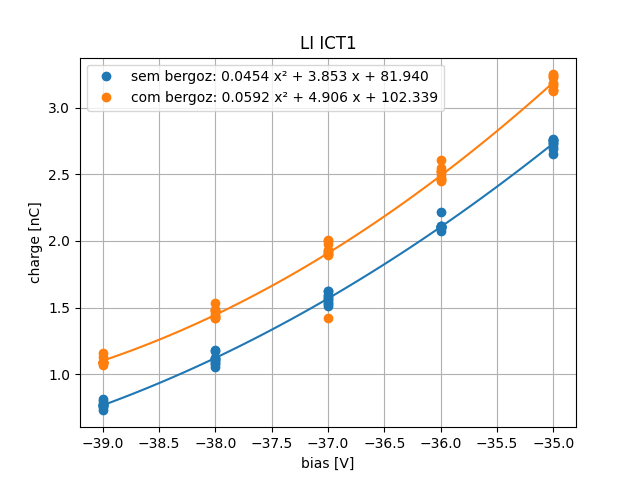
\includegraphics[width=\textwidth]{2024-05-31/figures/li-ict1.png}
        \caption{Calibration of LI ICT1.}
        \label{fig:a}
    \end{minipage}
    \hspace{0.5cm}
    \begin{minipage}[b]{0.45\linewidth}
        \centering
        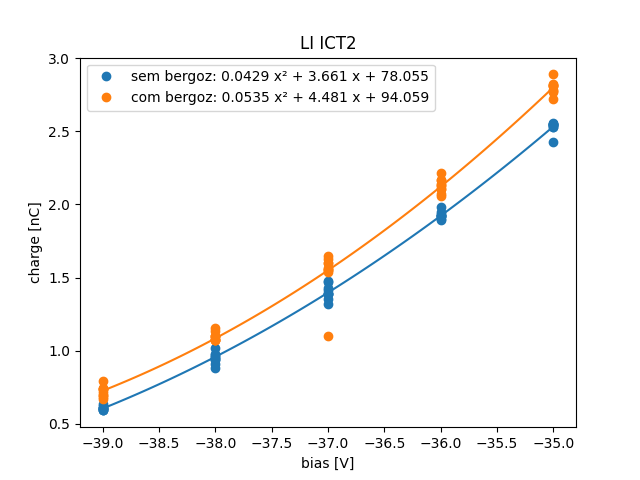
\includegraphics[width=\textwidth]{2024-05-31/figures/li-ict2.png}
        \caption{Calibration of LI ICT2.}
        \label{fig:b}
    \end{minipage}
\end{figure}
\end{frame}

\begin{frame}{Melhorias dos ICTs do LI, TB e TS}
\vspace{0.2cm}
Medidas de resistência de aterramento
\vspace{0.2cm}
{\footnotesize
\begin{itemize}
    \setlength\itemsep{1em}
    \item Entre barras de aterramento no LI, 1 Ohm,
    \item Entre barras e estrutura aceleradora, oscilando em torno de 1.2 Ohm
    \item A barra de aterramento próxima ao BPM 1-02 da TB não há nada conectado a ela e ela também não está aterrada.
    \item As medidas de resistência da câmara do booster em relação ao aterramento variam em torno 1.4 Ohm em trechos distintos 
aumentando até 6 Ohm quando se afasta do trecho de injeção, onde os magnetos pulsados estão conectados ao aterramento.
    \item Próximo ao trecho 04 do anel, tem um cabo que vem da sala de racks e está conectado ao aterramento sem um terminal, parecendo
    precária a conexão.
    \item A resistência entre anel e booster, variam entre 2 e 6 Ohm, diminuido nas proximidades onde o booster etá aterrado.
\end{itemize}
}
\end{frame}

\begin{frame}{Melhorias dos ICTs do LI, TB e TS}
\vspace{0.2cm}
Ruídos
\vspace{0.2cm}
\begin{itemize}
    \setlength\itemsep{1em}
    \item Fizemos diversas medidas do ruído induzido pelo septum, e os ICT's:
    \item Desconectamos o cabo de cada ICt separadamente, com o ímã pulsando e nenhum sinal do pulsador foi observado, conectando
    ou não ma malha externa do cabo coaxial. Mostrando que não é um sinal irradiado.
     \item Deconectamos todos os cabos inclusive os de sincronismo e conexão com a ethernet, e o sinaldo pulsador pode ainda ser observado
\end{itemize}
\end{frame}



%====================================================================
\section{Estimativa de corrente máxima}

\begin{frame}{Estimativa de corrente máxima}

{\footnotesize
\begin{itemize}
    % \setlength\itemsep{1em}
    \item Estudo dia 2024-05-13
\end{itemize}
}
% \begin{figure}[ht]
%     \begin{minipage}[b]{0.45\linewidth}
%         \centering
%         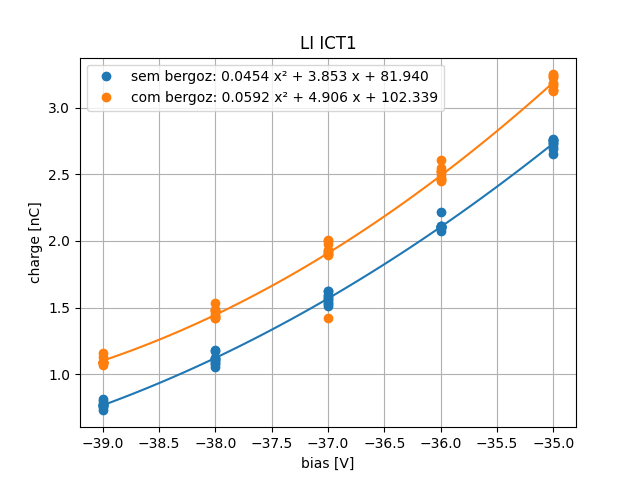
\includegraphics[width=\textwidth]{2024-05-31/figures/li-ict1.png}
%         \caption{Calibration of LI ICT1.}
%         \label{fig:a}
%     \end{minipage}
%     \hspace{0.5cm}
%     \begin{minipage}[b]{0.45\linewidth}
%         \centering
%         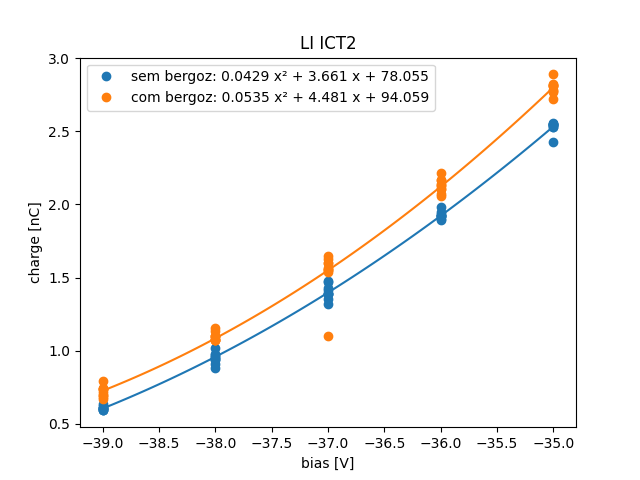
\includegraphics[width=\textwidth]{2024-05-31/figures/li-ict2.png}
%         \caption{Calibration of LI ICT2.}
%         \label{fig:b}
%     \end{minipage}
% \end{figure}
\end{frame}



%====================================================================
\section{FF de órbita para perturbação em 60 Hz}

\begin{frame}{FF de órbita para perturbação em 60 Hz}

\begin{itemize}
    \setlength\itemsep{1em}
    \item Estudos em 2024-05-14
\end{itemize}

\end{frame}



%====================================================================


%====================================================================
\section{Scan de delays dos pingers e testes de aquisição TbT}
\begin{frame}{testes com pingers}

{\footnotesize
\begin{itemize}
    \item estudo dia 2024-05-21
    \item amplitudes menores do que esperadas no feixe quando kickado pelos pingers
    \item desconfiando da temporização, fizemos scan dos \texttt{delay\_raw} para pingh e pingv
    \item delays ótimos encontrados, problema de amplitudes permaneceu
    \item realizamos aquisições varrendo kicks para levantar uma tabela de calibração 
    \item fator de calibração p/ (pingh, pingv) = (1.5417, 1.0227)
\end{itemize} 
}
\begin{minipage}{0.49\textwidth}
    \centering
    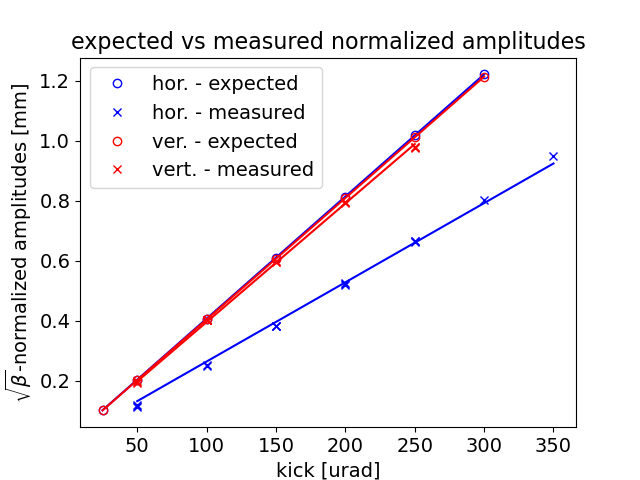
\includegraphics[width=0.9\columnwidth]{2024-06-21/figures/norm_amp_expected_vs_observed-210524.png}
    % \caption{pré-calibração}
\end{minipage}
\hfill
\begin{minipage}{0.49\textwidth}
    \centering
    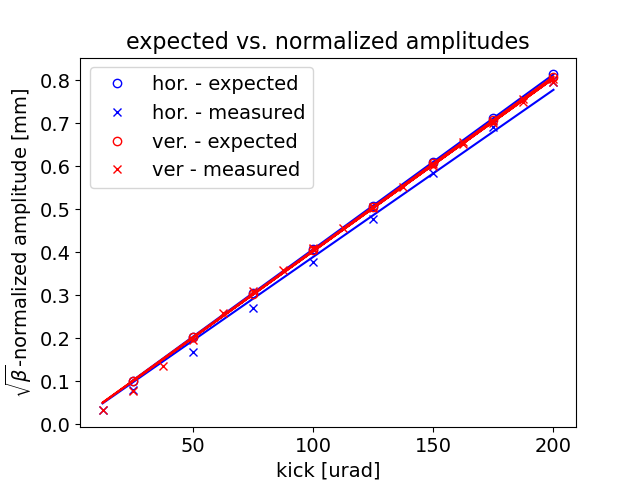
\includegraphics[width=0.9\columnwidth]{2024-06-21/figures/norm_amp_expected_vs_observed_post_calibration.png}
    % \caption{pós-calibração}
\end{minipage}
\end{frame}
%====================================================================
\section{otimização da injeção no booster}
\begin{frame}{otimização da injeção no Booster}
\begin{itemize}
    \item estudo dia 2024-05-27
    \item pós-otimização de amplitude e fase do subharmonic buncher 
    \item otimização da corrente na rampa do BO à baixa energia usando o RCDS
    \item botões de otimização
    \begin{itemize}
        \item PosAng na TB, BOInjKicker, kly2 amp, kly2 phase (rodadas 1 e 2)
        \item PosAng na TB, BOInjKicker, kly2 amp, kly2 phase, RF bottom phase (rodada 3)
    \end{itemize}
    \item Função objetivo: corrente à baixa energia (indice 60 da wfm) 
    \item Resultados
    
\end{itemize}    
\end{frame}
%====================================================================
\section{medidas de tune-shifts com amplitude}
\begin{frame}{Medidas de tune-shifts com amplitude}

{\footnotesize
\begin{itemize}
    \item estudo dia 2024-06-11
    \item com forças dos pingers calibrados, realizamos aquisições TbT do feixe kickado
    \item obtenção de tunes via espectro dos modos $U$ do SVD da matriz história de $N$ voltas nos 160 BPMs $X = U \Sigma V^\intercal$, $X = [[x_{ij}], [y_{ij}]] \in \mathbb{R}^{N\times 320}$ (reocortar figura)
\end{itemize}
}
\begin{figure}
    \centering
    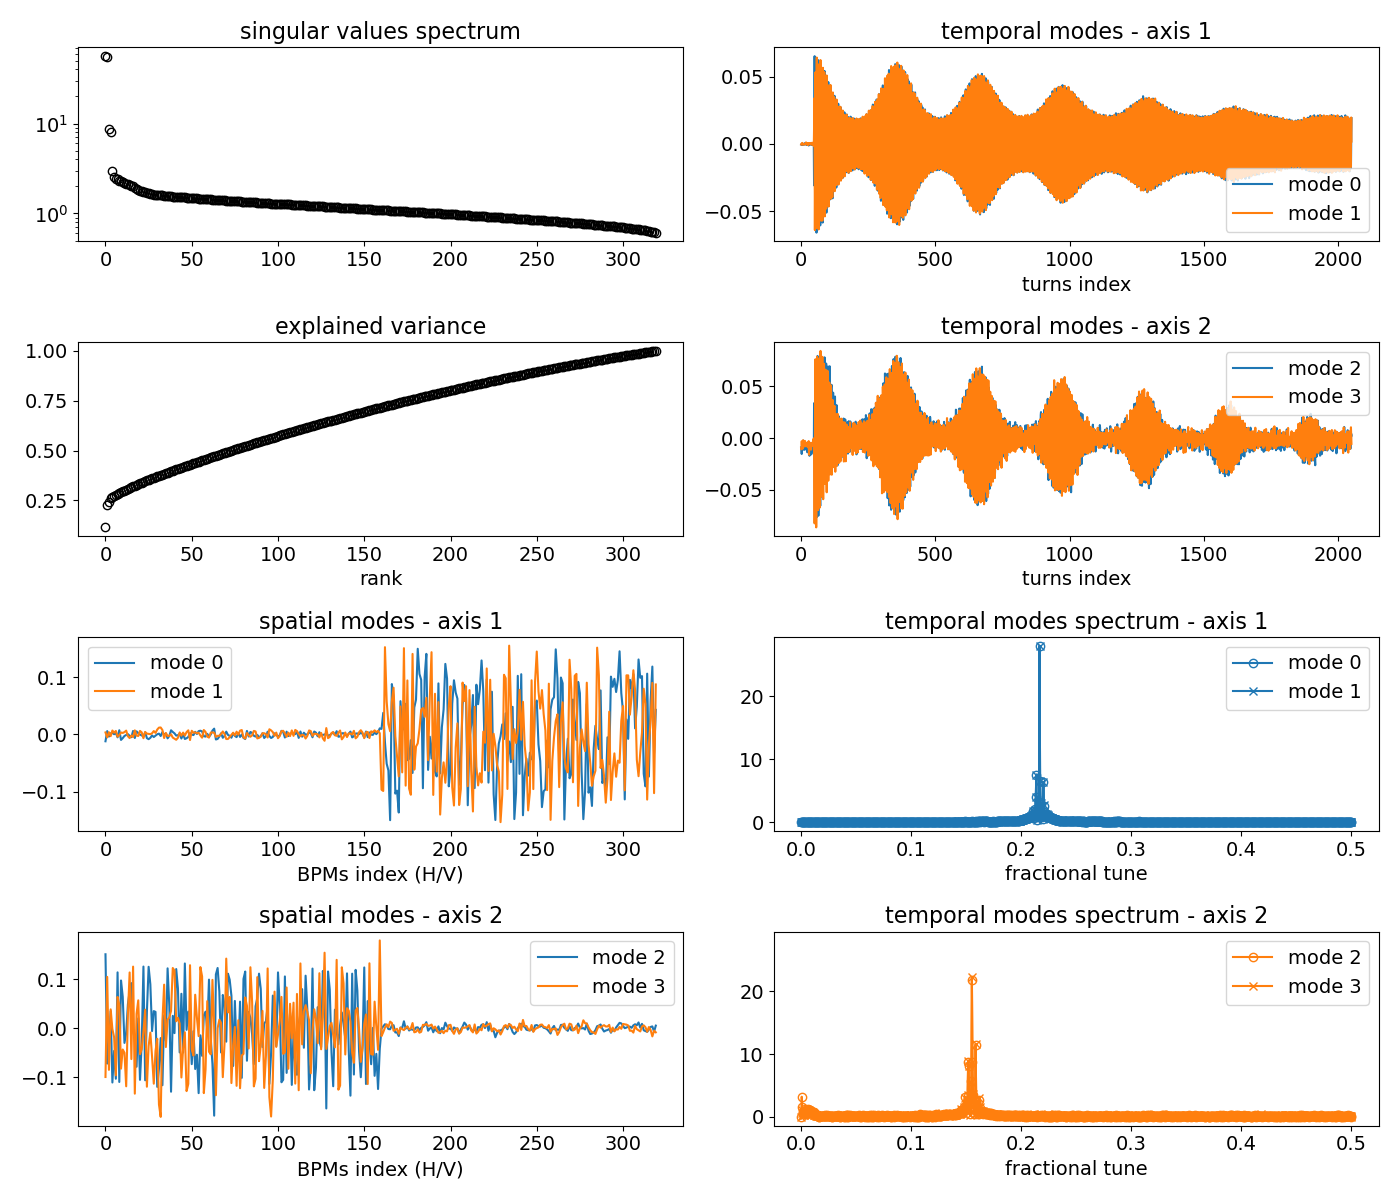
\includegraphics[scale=0.2]{2024-06-21/figures/tbt_modal_analysis.png}
\end{figure}
\end{frame}
\begin{frame}{medidas vs. modelo}
\begin{figure}
    \centering
    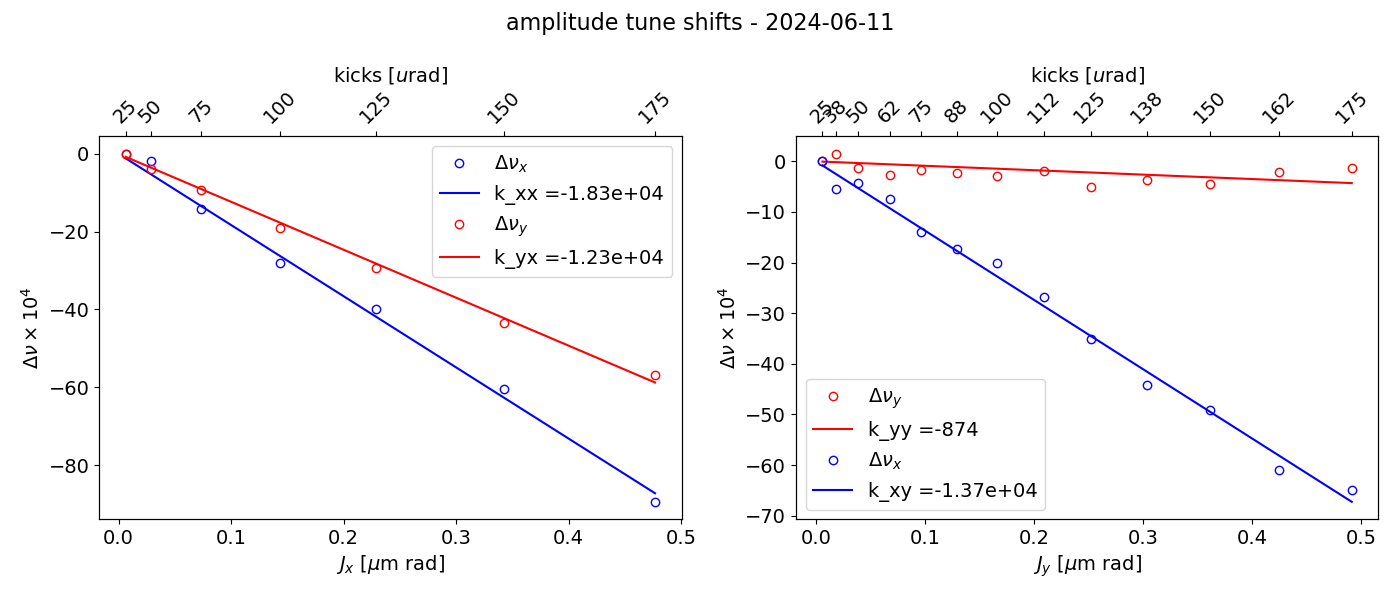
\includegraphics[scale=0.25]{2024-06-21/figures/adts110624.png}
\end{figure}
\begin{figure}
    \centering
    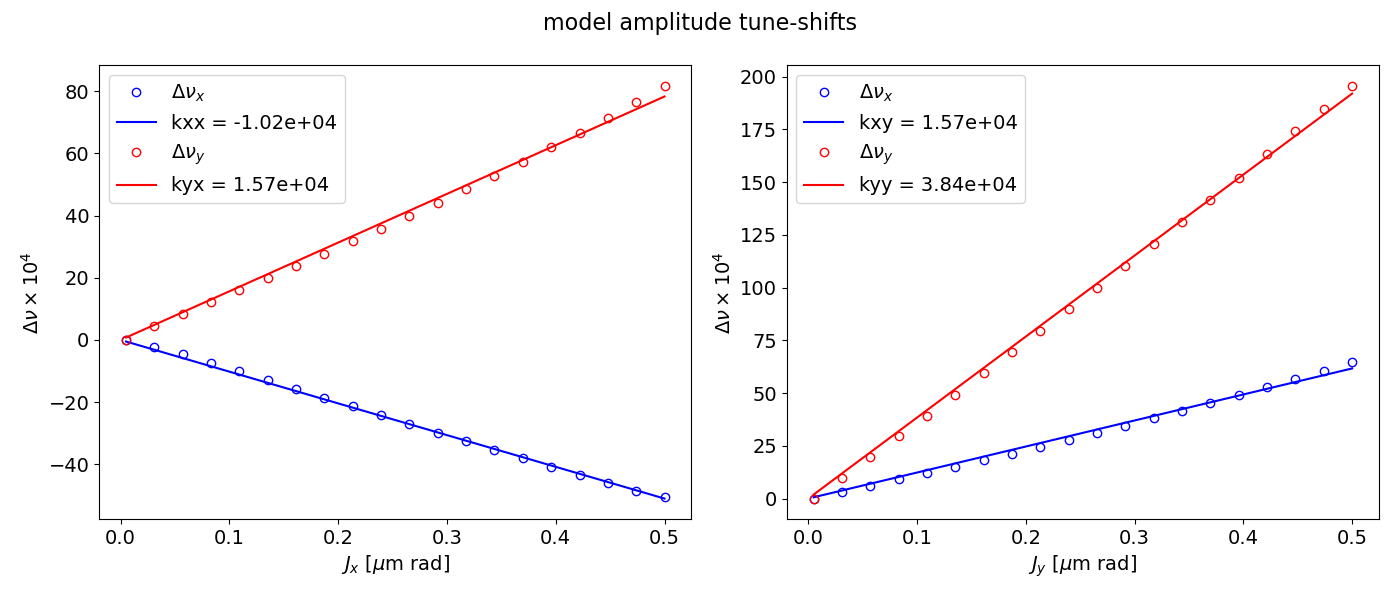
\includegraphics[scale=0.25]{2024-06-21/figures/adts_model.png}
\end{figure}
    
\end{frame}
\end{document}